\documentclass[12pt]{article}
\renewcommand{\baselinestretch}{0.95}

\usepackage{sbc-template}
\usepackage{graphicx,url}
\usepackage[utf8]{inputenc}
\makeatletter\let\normalsfcodes\relax\makeatother
\usepackage[brazil]{babel}
\AtBeginDocument{\providecommand{\normalsfcodes}{}}
\usepackage{comment}
\usepackage{booktabs}
\usepackage{tabularx}
\usepackage{tikz}
\usepackage{amsmath}
\usepackage{amssymb}
\usepackage{capt-of}
\usepackage{enumitem}
\usepackage{subcaption}
\usepackage[table]{xcolor}
\usepackage{multirow}
\usepackage{pgfgantt}
\usepackage{listings}
\usetikzlibrary{arrows.meta, positioning, shapes.geometric, fit, backgrounds}
\makeatletter
\providecommand\normalsfcodes{%
  \sfcode`\.=\@m
  \sfcode`\?=\@m
  \sfcode`\!=\@m
  \sfcode`\:=\@m
  \sfcode`\;=\@m
}
\makeatother

\graphicspath{{figs/}}
\newcommand{\code}[1]{\texttt{#1}}
\newcommand{\arq}[1]{\path{#1}}
\newcommand{\proj}{APIDrift-SDD}
\def\UrlBreaks{\do\/\do-}
\newcommand{\repourl}{\url{https://github.com/L42Matheus/APIDrift-SDD}}

\lstset{basicstyle=\ttfamily\scriptsize, columns=fullflexible, keepspaces=true,
  frame=single, rulecolor=\color{gray!50}, backgroundcolor=\color{gray!5},
  literate={á}{{\'a}}1 {é}{{\'e}}1 {ê}{{\^e}}1 {ç}{{\c{c}}}1 {ã}{{\~a}}1 {õ}{{\~o}}1 {í}{{\'i}}1 {ó}{{\'o}}1 {ú}{{\'u}}1}

\title{\proj: IA Generativa no \textit{Pipeline} de Integração Contínua para Detectar a Deriva entre Contratos OpenAPI e Serviços Spring}

\author{Lucas Matheus Silva\inst{1}}
\address{Instituto Federal da Paraíba (IFPB)\\Laboratório de Inovação em Software (LIS)}

\begin{document}
\maketitle
\sloppy

%%%%%%%%%%%%%%%%%%%%%%%%%%%%%%%%%%%%%%
%%%%%%%%%%%% Abstract %%%%%%%%%%%%%%%%
%%%%%%%%%%%%%%%%%%%%%%%%%%%%%%%%%%%%%%
\begin{abstract}
In microservice infrastructures, the OpenAPI contract is an infrastructure artifact: client teams, API gateways and generated clients rely on it, while the behavior is defined by the service code. Both are maintained separately and drift apart as the API evolves: the code changes, a failing test is adjusted, the pipeline turns green, and the contract keeps promising the old behavior. This research proposal presents \textit{\proj}, a generative-AI-assisted continuous-integration gate that binds requirements, the OpenAPI contract and Spring/Java code through a versioned specification, and uses a large language model (LLM) to check whether the contract text and the code mean the same thing. In an exploratory mutation study on a Spring Boot service (19 changes, 49 automated tests), version checks detect 2 of 12 injected drifts, usual practices (schema checks and conformance tests) detect 6, and structural traceability detects 10. The two remaining drifts change meaning while keeping every check green; the LLM-based check catches both, reaching 12 of 12 with both Claude Opus 5.5 and GPT-5.5. Claude adds no false alarm, while GPT flags 6 of 7 benign changes. The results are small-scale and motivate a study on real open-source Spring projects.
\end{abstract}

%%%%%%%%%%%%%%%%%%%%%%%%%%%%%%%%%%%%%%
%%%%%%%%%%%% Resumo %%%%%%%%%%%%%%%%%%
%%%%%%%%%%%%%%%%%%%%%%%%%%%%%%%%%%%%%%
\begin{resumo}
Em infraestruturas de microsserviços, o contrato OpenAPI é um artefato de infraestrutura: dele dependem equipes consumidoras, \textit{gateways} de API e clientes gerados automaticamente, enquanto o comportamento é definido pelo código do serviço. Os dois são mantidos separadamente e se afastam à medida que a API evolui: o código muda, um teste que falhou é ajustado, o \textit{pipeline} fica verde e o contrato continua prometendo o comportamento antigo. Este projeto de pesquisa apresenta o \textit{\proj}, um portão de integração contínua assistido por IA generativa que amarra requisitos, contrato OpenAPI e código Spring/Java por meio de uma especificação versionada e usa um modelo de linguagem de grande escala (LLM) para verificar se o texto do contrato e o código dizem a mesma coisa. Num estudo exploratório de mutações sobre um serviço Spring Boot (19 alterações, 49 testes automatizados), a checagem de versões detecta 2 de 12 derivas injetadas, as práticas usuais (checagem de esquema e testes de conformidade) detectam 6 e a rastreabilidade estrutural detecta 10. As duas restantes mudam o sentido mantendo todas as checagens verdes; a verificação por LLM detecta ambas e chega a 12 de 12 com o Claude Opus 5.5 e com o GPT-5.5. O Claude não acrescenta alarmes falsos; o GPT acusa 6 de 7 mudanças benignas. Os resultados são de pequena escala e motivam um estudo sobre projetos Spring reais de código aberto.
\end{resumo}

%%%%%%%%%%%%%%%%%%%%%%%%%%%%%%%%%%%%%%
%%%%%%%%%%%% Seção 1  %%%%%%%%%%%%%%%%
%%%%%%%%%%%%%%%%%%%%%%%%%%%%%%%%%%%%%%
\section{Introdu\c{c}\~ao}
\label{sec1:intro}

A infraestrutura de software das organizações é hoje, em grande parte, um conjunto de microsserviços que se comunicam por APIs REST \cite{dragoni2017microservices,fielding2000rest} e chegam à produção por \textit{pipelines} de integração e entrega contínuas (CI/CD) \cite{shahin2017cicd}. Para que equipes diferentes consigam integrar seus sistemas sem ler o código umas das outras, cada API publica um \textit{contrato}, em geral no formato OpenAPI \cite{openapi303}, que descreve rotas, tipos de dados e, em texto, as regras de negócio que a API aplica. O contrato é um artefato de infraestrutura: além de ser a documentação que o consumidor lê, é a entrada de \textit{gateways} de API, de geradores de bibliotecas cliente, de servidores simulados e de testes automáticos. O código do serviço, por exemplo em Spring Boot, é o que de fato executa.

O problema é que contrato e código evoluem em ritmos diferentes. APIs mudam com frequência e essas mudanças afetam quem as consome \cite{lamothe2021apievolution,wang2014restevolution}; numerar versões é a prática mais comum para controlar a evolução \cite{serbout2023versioning}, e a documentação de APIs é conhecida por ficar incompleta, ambígua ou desatualizada \cite{uddin2015apidocfails,aghajani2019docissues}. Quando o código muda e o contrato não, ou o contrário, nada quebra: o serviço responde, os testes passam e o consumidor segue implementando o que o contrato promete. Neste projeto, essa situação é chamada de \textbf{deriva de coevolução}: especificação, contrato e código deixam de dizer a mesma coisa depois de uma mudança.

As práticas usuais ajudam só em parte. Gerar o contrato a partir do código mantém rotas e tipos alinhados, mas não o texto que descreve as regras. Testes de contrato e ferramentas de teste de APIs REST \cite{golmohammadi2023resttesting,atlidakis2019restler,arcuri2019evomaster,hatfield2022schemathesis} verificam a estrutura e as respostas, e testes podem ser ``consertados'' junto com o código. O que falta é verificar o \textit{significado}: se o que o contrato diz em linguagem natural é o que o código faz. Modelos de linguagem de grande escala (LLMs) já são usados para ler especificações de APIs e apoiar testes \cite{kim2024llmrest,huynh2026rbctest} e para detectar inconsistências entre código e documentação \cite{xu2025docprism,lee2025metamon}, o que torna essa verificação viável.

Este projeto propõe o \textit{\proj}, uma abordagem orientada por especificações (\textit{Spec-Driven Development}, SDD) para a engenharia de APIs: requisitos, contrato OpenAPI e código Java são amarrados por uma especificação versionada, e um portão no \textit{pipeline} de integração contínua só libera a mudança quando os três estão consistentes. A IA generativa atua nesse portão como um revisor automático, semelhante aos revisores de código baseados em LLMs que já começam a ser adotados na indústria \cite{cihan2025acr}, mas especializado em comparar o texto do contrato com o código. As verificações estruturais (versões, vínculos e marcas de integridade) são baratas e determinísticas; a verificação semântica com IA generativa cobre o que elas não alcançam. A pesquisa busca responder: \textit{até onde testes de contrato e rastreabilidade estrutural detectam a deriva entre contrato e código, e qual é o ganho e o custo de usar IA generativa para verificar o significado?}

As contribuições pretendidas são: (i) a caracterização da deriva de coevolução entre especificação, contrato OpenAPI e código, com uma taxonomia de tipos; (ii) um verificador em níveis cumulativos, que permite atribuir cada detecção a um mecanismo; (iii) uma verificação semântica assistida por LLM entre o texto do contrato e o código Java; e (iv) um estudo empírico, baseado em mutações e depois em projetos reais, sobre ganhos, custos e limites dessas verificações. O protótipo já implementa (ii), uma primeira versão de (iii) com dois LLMs e um estudo inicial (iv), descrito na Seção~\ref{sec5:preliminares}.

\textbf{Relação com o tema.} O projeto se insere na aplicação de IA generativa no suporte à engenharia de infraestrutura de software em três pontos: (i) o objeto verificado são contratos de APIs, que sustentam a comunicação entre serviços e a configuração de \textit{gateways}, bibliotecas cliente e testes; (ii) a verificação roda no \textit{pipeline} de CI/CD, como portão antes do \textit{merge} e do \textit{deploy}; e (iii) a IA generativa apoia o engenheiro lendo o contrato e o código, explicando cada divergência em linguagem natural e, na etapa prevista do plano de pesquisa, propondo a correção do contrato ou do código para revisão humana.

O texto está organizado assim: a Seção~\ref{sec2:problema} descreve o problema; a Seção~\ref{sec3:fundamentacao} apresenta a fundamentação; a Seção~\ref{sec3:trab_rel} discute trabalhos relacionados; a Seção~\ref{sec4:abordagem} descreve a abordagem; a Seção~\ref{sec5:preliminares} reporta a avaliação exploratória; a Seção~\ref{sec6:plano} apresenta as lacunas e o plano de pesquisa; a Seção~\ref{sec7:ameacas} discute ameaças à validade; e a Seção~\ref{sec8:final} conclui.

%%%%%%%%%%%%%%%%%%%%%%%%%%%%%%%%%%%%%%
%%%%%%%%%%%% Seção 2  %%%%%%%%%%%%%%%%
%%%%%%%%%%%%%%%%%%%%%%%%%%%%%%%%%%%%%%
\section{O Problema: Deriva entre Contrato e Código}
\label{sec2:problema}

\textbf{Exemplo motivador.} Considere uma API de decisões de reembolso de uma plataforma fictícia de pedidos, implementada em Spring Boot, com a rota \code{POST /reembolsos/decisoes}. O aplicativo do cliente e o sistema de atendimento, mantidos por outras equipes, consomem essa API a partir do contrato OpenAPI. Na versão 2 da política, a empresa criou uma exceção: o cliente \textit{premium} pode cancelar com reembolso até 1~hora após o despacho. O requisito REQ-05, o texto do contrato e o código dizem a mesma coisa (Figura~\ref{fig:codigo}).

\begin{figure}[!ht]
\centering
\begin{minipage}{0.48\linewidth}
\begin{lstlisting}
# openapi.yaml (contrato v2)
tags:
- name: cancelamento
  description: 'Cancelamento antes do
    despacho é permitido. Após despacho,
    normalmente é negado; exceção: cliente
    premium que cancela até 1 hora depois
    do despacho (inclusive) pode ser
    reembolsado, salvo fraude ou falha
    prioritária.'
  x-apidrift:
    policy-version: '2'
    requirement_ids:
      [REQ-03, REQ-04, REQ-05]
    rule_fingerprints:
      REG-PREMIUM-EXC: 9f1c...
\end{lstlisting}
\end{minipage}\hfill
\begin{minipage}{0.5\linewidth}
\begin{lstlisting}
// PoliticaReembolso.java (serviço Spring)
@RegraPolitica(id = "REG-PREMIUM-EXC",
    prioridade = 25,
    requisitos = {"REQ-05"},
    decisao = Decisao.PERMITIR,
    justificativa = "Exceção premium: pedido
      cancelado até 1 hora após despacho.")
boolean excecaoPremium(Solicitacao s) {
  return TRUE.equals(s.cancelamentoCliente())
    && TRUE.equals(s.despachado())
    && TRUE.equals(s.clientePremium())
    && s.horasAposDespacho() != null
    && s.horasAposDespacho() <= 1.0;
}
\end{lstlisting}
\end{minipage}
\caption{A mesma regra no contrato OpenAPI (texto lido pelos consumidores) e no código Java (o que executa).}
\label{fig:codigo}
\end{figure}

Meses depois, um desenvolvedor altera o limiar para 2~horas, sem que a política tenha mudado. O teste de conformidade do caso ``\textit{premium}, 1,5~hora após o despacho'' falha, e o desenvolvedor ajusta a decisão esperada para que o \textit{pipeline} volte a ficar verde. A Figura~\ref{fig:problema} mostra o resultado: a API passa a aprovar reembolsos que o requisito e o contrato dizem que não existem, e o aplicativo, construído a partir do contrato, continua dizendo ao cliente que o prazo é de 1~hora. Nenhum teste falha e nenhum alerta é emitido.

\begin{figure}[!ht]
\centering
\resizebox{0.82\linewidth}{!}{
\begin{tikzpicture}[
  box/.style={rectangle, draw=blue!60, fill=blue!8, rounded corners=5pt, text centered,
    minimum height=1.1cm, text width=5.0cm, font=\small, line width=0.7pt},
  old/.style={box, draw=gray!70, fill=gray!10},
  bad/.style={box, draw=red!60, fill=red!6, text width=5.6cm},
  chg/.style={box, draw=orange!70, fill=orange!10, text width=5.2cm},
  arrow/.style={->, >=Stealth, thick, color=gray!60}
]
\node[chg] (mud) at (0,0) {\textbf{Mudança no código}\\ limiar \textit{premium}: 1h $\rightarrow$ 2h\\ teste ajustado para passar};
\node[box] (cod) at (3.4,-2.6) {\textbf{Serviço Spring} (alterado)\\ \code{horasAposDespacho() <= 2.0}\\ \textit{pipeline} verde};
\node[old, text width=5.4cm] (ctr) at (-3.6,-2.6) {\textbf{Contrato OpenAPI} (inalterado)\\ ``\textit{premium} pode cancelar\\ até 1 hora''};
\node[box, text width=4.6cm] (cli) at (0,-5.2) {\textbf{Cliente \textit{premium}}\\ cancela 1,5 h após o despacho};
\node[bad] (dec) at (0,-7.6) {\textbf{API: PERMITIR}\\ Contrato e aplicativo: ``prazo de 1 h''\\ REQ-05: ``até 1 hora''};
\node[align=left, font=\small, text width=4.2cm, anchor=west] (obs) at (3.1,-7.5) {Sem erro, sem alerta:\\ o contrato promete uma\\ coisa e a API faz outra.};

\draw[arrow] (mud) -- node[above right, font=\footnotesize, color=black]{alterado} (cod);
\draw[arrow, dashed] (mud) -- node[above left, font=\footnotesize, color=black]{esquecido} (ctr);
\draw[arrow] (ctr) -- node[below left, font=\footnotesize, color=black]{lido pelo consumidor} (cli);
\draw[arrow] (cod) -- node[below right, font=\footnotesize, color=black]{executa} (cli);
\draw[arrow] (cli) -- (dec);
\end{tikzpicture}}
\caption{Deriva de coevolução: o código muda, o teste é ajustado e o contrato continua descrevendo o comportamento antigo.}
\label{fig:problema}
\end{figure}

\textbf{Tipos de deriva.} O exemplo é um de vários casos. A Tabela~\ref{tab:tipos_deriva} resume os tipos considerados, que orientam o estudo de mutações da Seção~\ref{sec5:preliminares}.

\begin{table}[!ht]
\centering
\caption{Tipos de deriva de coevolução entre especificação, contrato e código.}
\label{tab:tipos_deriva}
\small
\begin{tabularx}{\linewidth}{l X X}
\toprule
\textbf{Tipo} & \textbf{O que acontece} & \textbf{Efeito} \\
\midrule
Código sem contrato & o código muda (limiar, precedência, decisão) e o texto do contrato não & a API faz algo que o contrato não diz \\
Contrato sem código & o texto do contrato muda e o código não & consumidores implementam um comportamento que não existe \\
Atualização parcial & parte do contrato fica na versão anterior & documentação de versões misturadas \\
Requisito órfão & um requisito é criado ou removido sem regra correspondente & comportamento sem respaldo no requisito \\
Deriva ressincronizada & o sentido muda e testes ou marcas de controle são ajustados sem revisão real & passa por qualquer checagem estrutural \\
\bottomrule
\end{tabularx}
\end{table}

\textbf{Por que as práticas usuais não bastam.} O versionamento semântico do contrato detecta apenas o caso em que as versões declaradas diferem. A checagem de esquema e a geração do contrato a partir do código alinham rotas e tipos, mas não o texto que descreve as regras. Testes de conformidade detectam a mudança de comportamento enquanto ninguém os altera; quando o teste é ajustado junto com o código, como no exemplo, eles passam a confirmar a deriva. O problema exige verificar o \textit{vínculo} entre requisito, contrato e código a cada mudança, e não cada artefato isoladamente.

%%%%%%%%%%%%%%%%%%%%%%%%%%%%%%%%%%%%%%
%%%%%%%%%%%% Seção 3  %%%%%%%%%%%%%%%%
%%%%%%%%%%%%%%%%%%%%%%%%%%%%%%%%%%%%%%
\section{Fundamentação}
\label{sec3:fundamentacao}

\textbf{APIs REST, contratos e evolução.} O estilo REST \cite{fielding2000rest} organiza a comunicação entre serviços em recursos e operações sobre HTTP, e a especificação OpenAPI \cite{openapi303} descreve essas operações num documento legível por máquinas e por pessoas, que inclui descrições em linguagem natural e extensões próprias (\code{x-}). A evolução de APIs é um tema amplo da Engenharia de Software \cite{lamothe2021apievolution}: mudanças em APIs REST exigem adaptação dos clientes \cite{wang2014restevolution}, e o versionamento é a principal forma de comunicá-las \cite{serbout2023versioning}. Em contratos dirigidos pelo consumidor, os clientes declaram o que esperam do serviço e o provedor verifica essas expectativas a cada mudança \cite{robinson2006cdc}.

\textbf{Documentação de APIs.} Documentação incorreta, incompleta ou desatualizada está entre os problemas mais citados por quem consome APIs \cite{uddin2015apidocfails,aghajani2019docissues}, e alguns desses problemas podem ser detectados automaticamente como \textit{smells} de documentação \cite{khan2021docsmells}. De forma mais geral, artefatos acoplados tendem a divergir quando evoluem em ritmos diferentes, como código e comentários \cite{tan2007icomment,wen2019codecomment} ou código e testes \cite{zaidman2011coevolution,lehman1980laws}.

\textbf{Especificações como fonte de verdade.} Projeto por contrato \cite{meyer1992dbc} e engenharia dirigida por modelos \cite{schmidt2006mde} defendem especificações explícitas e verificáveis como fonte do comportamento do software. O SDD retomou esse princípio para guiar agentes de codificação a partir de especificações versionadas \cite{githubspeckit2025}. A rastreabilidade de requisitos liga cada requisito aos artefatos que o implementam \cite{gotel1994traceability,ramesh2001traceability}, e mantê-la atualizada continua sendo um desafio \cite{clelandhuang2014traceability}.

\textbf{LLMs na engenharia de software e teste de mutação.} LLMs vêm sendo aplicados a várias tarefas de Engenharia de Software \cite{hou2024llm4se,fan2023llmse}, e um LLM pode atuar como avaliador de textos \cite{zheng2023judge}, desde que suas respostas sejam validadas. O teste de mutação avalia a capacidade de detecção de um conjunto de verificações injetando defeitos artificiais \cite{demillo1978hints,jia2011mutation,papadakis2019mutation}; a definição do que conta como defeito exige um oráculo \cite{barr2015oracle}. Aqui, os operadores de mutação injetam derivas em código, testes, contrato e especificação, e medem se cada nível do verificador as detecta.

%%%%%%%%%%%%%%%%%%%%%%%%%%%%%%%%%%%%%%
%%%%%%%%%%%% Seção 4  %%%%%%%%%%%%%%%%
%%%%%%%%%%%%%%%%%%%%%%%%%%%%%%%%%%%%%%
\section{Trabalhos Relacionados}
\label{sec3:trab_rel}

\textbf{Teste de APIs REST.} Ferramentas como RESTler \cite{atlidakis2019restler}, EvoMaster \cite{arcuri2019evomaster} e Schemathesis \cite{hatfield2022schemathesis} usam o contrato OpenAPI para gerar requisições e encontrar falhas no serviço; o levantamento de \cite{golmohammadi2023resttesting} organiza essa área. Elas verificam se o serviço respeita a \textit{estrutura} do contrato (tipos, códigos de \textit{status}), não se o texto do contrato descreve as regras que o código aplica. Contratos dirigidos pelo consumidor \cite{robinson2006cdc} verificam exemplos de interação, que precisam ser mantidos à mão e podem ser ajustados junto com o código.

\textbf{LLMs aplicados a especificações de APIs.} \cite{kim2024llmrest} usam LLMs para extrair restrições e valores das descrições em linguagem natural do contrato e melhorar o teste de APIs REST. O RBCTest \cite{huynh2026rbctest} minera, com LLMs, restrições sobre o corpo das respostas a partir da especificação e encontra divergências entre especificação e respostas reais. O SpeCrawler \cite{lazar2024specrawler} gera contratos OpenAPI a partir de documentação \textit{online}, e o Hermes \cite{lima2026hermes} usa um sistema multiagente de LLMs para encontrar \textit{smells} de documentação em contratos OpenAPI. Nenhum deles compara o texto do contrato com o código-fonte da implementação, nem acompanha a evolução entre versões.

\textbf{Inconsistência entre código e documentação.} DocPrism \cite{xu2025docprism} e METAMON \cite{lee2025metamon} usam LLMs para detectar divergências entre código e documentação de funções; o MPDetector \cite{xu2024mpdetector} combina execução simbólica e LLMs para comparar restrições entre parâmetros no código e na documentação de bibliotecas Python. São a base mais próxima da verificação semântica proposta aqui, mas tratam documentação de funções, não contratos de serviços, e analisam uma única versão.

\textbf{Lacuna.} A Tabela~\ref{tab:relacionados} resume a comparação. Nenhum dos trabalhos verifica, ao mesmo tempo, o esquema e o texto do contrato contra o código da implementação, ao longo da evolução de versões e como portão de integração contínua. Essa combinação é o foco do \proj. A revisão sistemática prevista na Seção~\ref{sec6:plano} \cite{kitchenham2007slr} confirmará ou refinará essa lacuna.

\begin{table}[!ht]
\centering
\caption{Comparação com trabalhos relacionados (\checkmark: trata; $\sim$: parcialmente; --: não trata).}
\label{tab:relacionados}
\small
\resizebox{\linewidth}{!}{%
\begin{tabular}{l c c c c c}
\toprule
\textbf{Trabalho} & \textbf{Esquema} & \textbf{Texto do} & \textbf{Código-} & \textbf{Evolução} & \textbf{Usa} \\
 & \textbf{do contrato} & \textbf{contrato} & \textbf{fonte} & \textbf{de versões} & \textbf{LLM} \\
\midrule
\cite{atlidakis2019restler,arcuri2019evomaster,hatfield2022schemathesis} & \checkmark & -- & $\sim$ & -- & -- \\
\cite{robinson2006cdc} & \checkmark & -- & $\sim$ & \checkmark & -- \\
\cite{kim2024llmrest,huynh2026rbctest} & \checkmark & \checkmark & -- & -- & \checkmark \\
\cite{lazar2024specrawler,lima2026hermes} & \checkmark & \checkmark & -- & -- & \checkmark \\
\cite{xu2025docprism,lee2025metamon,xu2024mpdetector} & -- & $\sim$ & \checkmark & -- & \checkmark \\
\textbf{\proj} & \checkmark & \checkmark & \checkmark & \checkmark & \checkmark \\
\bottomrule
\end{tabular}}
\end{table}

%%%%%%%%%%%%%%%%%%%%%%%%%%%%%%%%%%%%%%
%%%%%%%%%%%% Seção 5  %%%%%%%%%%%%%%%%
%%%%%%%%%%%%%%%%%%%%%%%%%%%%%%%%%%%%%%
\section{Abordagem Proposta}
\label{sec4:abordagem}

\textbf{Artefatos.} Cada versão da API reúne quatro artefatos que precisam coevoluir: (i) a \textit{especificação} versionada (\arq{api/spec/vN/specification.yaml}), com requisitos de identificador estável e critério de aceitação, um índice de regras (prioridade, decisão, requisitos atendidos e seção do contrato que as documenta) e o \textit{digest} SHA-256 \cite{nist2015sha} do texto aprovado de cada seção do contrato; (ii) o \textit{contrato OpenAPI} (\arq{api/contracts/vN/openapi.yaml}), em que cada \textit{tag} descreve em texto uma parte da política e guarda, na extensão \code{x-apidrift}, a versão da política, os requisitos citados e a marca de integridade (\textit{fingerprint}) de cada regra Java que descreve; (iii) o \textit{código} do serviço Spring Boot, em que cada regra é um método anotado com \code{@RegraPolitica} (Figura~\ref{fig:codigo}) e as regras são avaliadas em ordem de prioridade; e (iv) os \textit{testes de conformidade}, casos rotulados executados com JUnit no \code{mvn test}. O \textit{fingerprint} de uma regra é calculado sobre os atributos da anotação e o corpo do método sem comentários e sem espaços irrelevantes, de modo que reformatar ou comentar o código não o altera, mas mudar lógica, decisão, prioridade ou justificativa, sim.

\textbf{Portão de integração contínua.} A Figura~\ref{fig:pipeline} mostra o fluxo. A cada \textit{pull request} que altera o contrato, a especificação ou o código, o verificador executa os níveis em sequência e só libera a mudança se nenhum deles apontar divergência (política \textit{fail-closed}); caso contrário, a mudança volta para revisão com a lista de problemas, cada um com sua categoria. Depois que uma pessoa revisa e aprova a mudança, as marcas são recalculadas (\code{apidrift fingerprint --write}) e entram no mesmo \textit{commit}. O protótipo traz esse portão como uma \textit{GitHub Action}.

\begin{figure}[!ht]
\centering
\resizebox{\linewidth}{!}{
\begin{tikzpicture}[
  box/.style={rectangle, draw=blue!60, fill=blue!8, rounded corners=5pt, text centered,
    minimum height=1.25cm, text width=2.6cm, font=\small, line width=0.7pt},
  art/.style={box, draw=gray!70, fill=gray!10, minimum height=0.7cm, text width=2.6cm},
  ai/.style={box, draw=orange!70, fill=orange!10},
  alert/.style={box, draw=red!60, fill=red!6, text width=3.0cm},
  ok/.style={box, draw=green!50!black, fill=green!6, text width=3.0cm},
  arrow/.style={->, >=Stealth, thick, color=gray!60},
  lbl/.style={font=\footnotesize, color=black, fill=white, inner sep=1pt}
]
\node[art] (spec) at (0,1.0)  {Especificação};
\node[art] (oas)  at (0,0)    {Contrato OpenAPI};
\node[art] (java) at (0,-1.0) {Código Java e testes};
\node[box] (l1) at (3.5,0)  {\textbf{L1}\\ versões\\ declaradas};
\node[box] (l2) at (6.6,0)  {\textbf{L2}\\ esquema e testes\\ de conformidade};
\node[box] (l3) at (9.7,0)  {\textbf{L3}\\ rastreabilidade\\ SDD (marcas)};
\node[ai]  (l4) at (12.8,0) {\textbf{L4}\\ IA: contrato e\\ código dizem o mesmo?};
\node[ok]    (ok)  at (16.4,0.8)  {\textbf{\textit{Merge} e \textit{deploy}}};
\node[alert] (blk) at (8.15,-2.6) {\textbf{Bloqueio}\\ e revisão humana};
\draw[arrow] (spec.east) -- (l1.west |- spec.east);
\draw[arrow] (oas) -- (l1);
\draw[arrow] (java.east) -- (l1.west |- java.east);
\draw[arrow] (l1) -- (l2); \draw[arrow] (l2) -- (l3); \draw[arrow] (l3) -- (l4);
\draw[arrow] (l4.east) -- node[lbl, above]{ok} (ok.west);
\foreach \n in {l1,l2,l3,l4} \draw[arrow, color=red!40] (\n.south) -- (blk.north -| \n.south) ;
\draw[thick, color=red!40] (l1.south |- blk.north) ++(0,0.35) -- ([yshift=0.35cm]l4.south |- blk.north);
\end{tikzpicture}}
\caption{O verificador como portão de integração contínua: cada nível acrescenta categorias de verificação; qualquer divergência bloqueia a mudança.}
\label{fig:pipeline}
\end{figure}

\textbf{Níveis de verificação.} Para que cada detecção possa ser atribuída a um mecanismo, cada problema pertence a uma categoria, e os níveis ativam subconjuntos cumulativos dessas categorias (Tabela~\ref{tab:niveis}). L1 representa o versionamento convencional; L2 acrescenta o que equipes de API costumam fazer, isto é, comparar o esquema do contrato com os tipos Java (\code{record Solicitacao} e \code{enum Decisao}) e rodar os testes de conformidade compilando o pacote de política com \code{javac}; L3 acrescenta a rastreabilidade SDD; e L4, a verificação semântica. Os ganhos atribuíveis à proposta são, portanto, as diferenças entre L2 e L3/L4.

\begin{table}[!ht]
\centering
\caption{Níveis cumulativos do verificador.}
\label{tab:niveis}
\small
\begin{tabularx}{0.97\linewidth}{l l X}
\toprule
\textbf{Nível} & \textbf{Categorias ativas} & \textbf{Interpretação} \\
\midrule
L0 & nenhuma & sem portão \\
L1 & estrutura, versão & versionamento convencional \\
L2 & + esquema, conformidade & práticas usuais: esquema do contrato e testes \\
L3 & + IDs, referências, \textit{fingerprint}, \textit{digest}, cobertura & rastreabilidade SDD entre requisito, contrato e código \\
L4 & + semântica (LLM) & o texto do contrato e o código dizem o mesmo? \\
\bottomrule
\end{tabularx}
\end{table}

\textbf{Verificação semântica (L4).} Para cada seção (\textit{tag}) do contrato, o LLM recebe o texto da seção, o código-fonte Java dos métodos que ela documenta (anotação e corpo), os requisitos ligados e a lista de todas as regras por prioridade, também com código. A instrução explica que a primeira regra verdadeira decide, para que uma exclusão citada no texto (por exemplo, fraude) seja reconhecida quando outra regra já a decide antes, e pede que diferenças de redação, estilo ou nomes de variáveis sejam ignoradas. A resposta segue um esquema JSON fixo: se a seção é consistente e, para cada divergência, a regra, o aspecto afetado (limiar, decisão, condição, exceção, precedência ou requisito) e uma explicação. A verificação é \textit{fail-closed}: recusa, falha de rede ou resposta fora do esquema geram alerta, nunca aprovação. O protótipo aceita Claude (Anthropic) e GPT (OpenAI) pelos SDKs oficiais e guarda cada resposta num \textit{cache} indexado pelo \textit{hash} do pedido, o que permite repetir o experimento sem novas chamadas.

\textbf{Papel da IA.} O LLM não decide nada em produção e não altera artefatos: ele é um revisor automático que só atua no portão, antes do \textit{merge}, e cuja resposta é tratada como um alerta para revisão humana. Isso limita o efeito de erros do modelo a alarmes falsos ou derivas não apontadas, que são justamente o que a avaliação mede.

%%%%%%%%%%%%%%%%%%%%%%%%%%%%%%%%%%%%%%
%%%%%%%%%%%% Seção 6  %%%%%%%%%%%%%%%%
%%%%%%%%%%%%%%%%%%%%%%%%%%%%%%%%%%%%%%
\section{Avaliação Exploratória}
\label{sec5:preliminares}

\textbf{Configuração.} O serviço de exemplo usa Spring Boot 3.3 e Java 21, com cinco regras de reembolso e cancelamento, 18 casos de conformidade rotulados e um teste da rota com MockMvc (19 testes JUnit). A versão 1 da API não tem a exceção \textit{premium}; a versão 2 a introduz por meio do requisito REQ-05 e da regra REG-PREMIUM-EXC. O verificador e o estudo de mutações estão no pacote Python \code{apidrift}, com 30 testes automatizados que simulam o LLM e rodam sem rede. Os níveis L0--L3 são determinísticos. O nível L4 usa o Claude Opus 5.5 (\code{claude-opus-5-5}) e o GPT-5.5 (\code{gpt-5.5}), com esforço de raciocínio \textit{medium} e saída em esquema JSON estrito, numa única execução em 12/11/2026. Os resultados não sustentam inferência estatística: o serviço é sintético, os mutantes e os rótulos foram escritos pelo próprio autor, há um mutante por tipo e cada modelo foi executado uma vez.

\textbf{Operadores de mutação.} Partindo da versão 2 sincronizada, doze operadores produzem derivas (M01--M12) e sete produzem mudanças benignas (N01--N07), com rótulo atribuído \textit{a priori} (Tabela~\ref{tab:mutantes}). Os operadores alteram o código Java, os testes, o contrato OpenAPI e a especificação, isolados ou em conjunto. Cada mutante é verificado nos cinco níveis. Para medir o efeito operacional, o código de cada mutante é compilado e executado sobre os 18 casos, e conta-se quantas decisões a API passaria a tomar de forma diferente da política vigente se a mudança fosse liberada.

\begin{table}[!ht]
\centering
\caption{Operadores de mutação (artefato alterado entre parênteses).}
\label{tab:mutantes}
\scriptsize
\begin{tabularx}{\linewidth}{l X l X}
\toprule
\textbf{ID} & \textbf{Deriva injetada} & \textbf{ID} & \textbf{Mudança benigna} \\
\midrule
M01 & limiar \textit{premium} 1h$\rightarrow$2h (código) & N01 & métodos de regra reordenados (código) \\
M02 & prioridade da exceção trocada (código) & N02 & seções reordenadas (contrato) \\
M03 & decisão invertida (código) & N03 & comentário e formatação (código) \\
M04 & método de regra removido (código) & N04 & metadados: contato e servidores (contrato) \\
M05 & requisito removido (especificação) & N05 & correção de pontuação (contrato) \\
M06 & requisito sem regra (especificação) & N06 & evolução completa e sincronizada (todos) \\
M07 & justificativa devolvida pela API contradiz o contrato (código) & N07 & refatoração: parâmetro renomeado (código) \\
M08 & seção do contrato na versão anterior (contrato) & & \\
M09 & texto do contrato perde a exceção (contrato) & & \\
M10 & M09 com marcas recalculadas (contrato) & & \\
M11 & M01 com teste ajustado e marcas recalculadas (código e testes) & & \\
M12 & contrato v1 inteiro com código v2 (contrato) & & \\
\bottomrule
\end{tabularx}
\end{table}

\textbf{Resultados por nível.} A Figura~\ref{fig:matriz} mostra o resultado mutante a mutante e a Figura~\ref{fig:sensibilidade} o agrega. O versionamento convencional (L1) detecta apenas as duas derivas que mudam a versão declarada (M08 e M12). As práticas usuais (L2) chegam a 6/12: os testes de conformidade pegam as quatro mudanças de comportamento no código (M01--M04). Elas não percebem nada que esteja só no contrato ou na especificação (M05, M06, M07 e M09), nem as duas derivas ressincronizadas (M10 e M11). A rastreabilidade SDD (L3) chega a 10/12: as marcas de integridade pegam a justificativa alterada (M07) e o texto editado sem revisão (M09), e os vínculos pegam os requisitos removido e órfão (M05 e M06). O custo são dois alarmes falsos em sete mudanças benignas: a correção de pontuação (N05) altera o \textit{digest} do texto, e o parâmetro renomeado (N07) altera o \textit{fingerprint} do método, embora o comportamento seja o mesmo.

\begin{figure}[!ht]
\centering
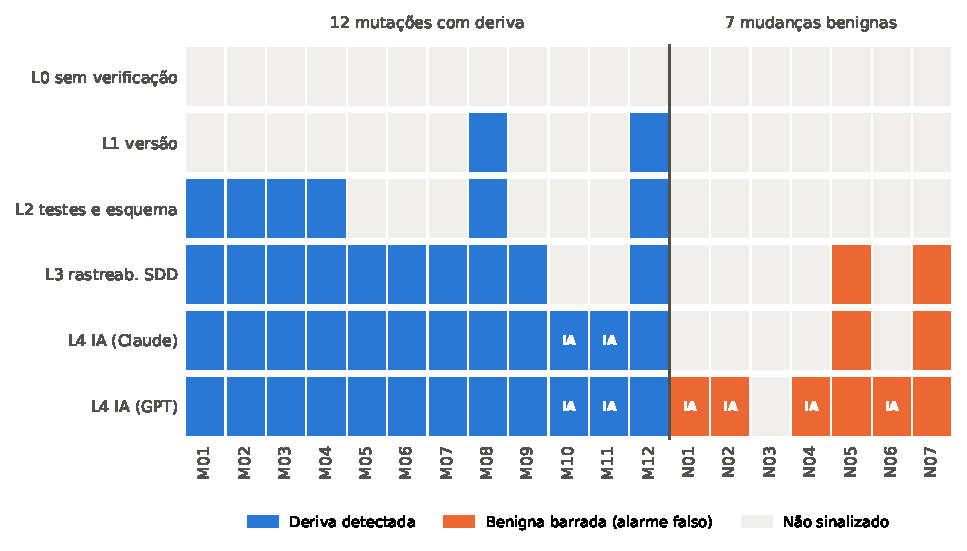
\includegraphics[width=0.95\linewidth]{fig_api_matriz.pdf}
\caption{Detecção por mutante e por nível do verificador. ``IA'' marca as células de L4 em que só a categoria semântica sinalizou.}
\label{fig:matriz}
\end{figure}

\begin{figure}[!ht]
\centering
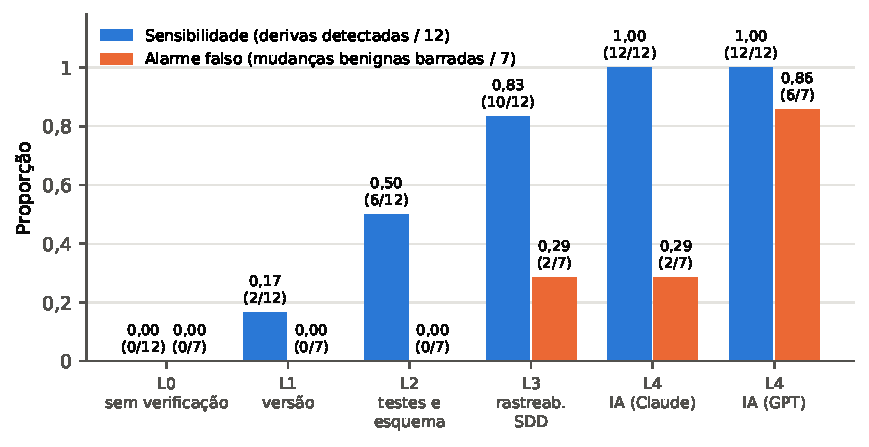
\includegraphics[width=0.9\linewidth]{fig_api_sensibilidade.pdf}
\caption{Sensibilidade e taxa de alarme falso por nível.}
\label{fig:sensibilidade}
\end{figure}

\textbf{O que só a IA detecta.} M10 e M11 passam por L0--L3. Em M10, o texto do contrato passa a dizer que todo cancelamento após o despacho é negado e as marcas são recalculadas; em M11, que é o exemplo da Seção~\ref{sec2:problema}, o limiar muda no código, o teste é ajustado e as marcas são recalculadas. A verificação estrutural é contornada por construção: \textit{fingerprints} e \textit{digests} atestam que os artefatos não mudaram desde a última aprovação, não que contrato e código dizem a mesma coisa. Os dois modelos detectam os dois casos. Em M10, apontam que o contrato omite a exceção \textit{premium} que o método \code{excecaoPremium} e o REQ-05 preveem; em M11, que o código usa \code{<= 2.0} enquanto o texto do contrato e o critério de aceitação dizem 1~hora. Com o Claude, a verificação semântica não produziu nenhum alarme falso nas sete mudanças benignas, incluindo a refatoração N07 e a evolução completa N06; os dois alarmes falsos de L4 são os mesmos herdados de L3.

\textbf{Os modelos diferem nas mudanças benignas.} O GPT acusou 6 das 7 mudanças benignas. Em cinco delas (N01, N02, N04, N05 e N07), o apontamento é o mesmo, e ele já aparece na versão 2 original, antes de qualquer mutação: o método \code{excecaoPremium} verifica \code{horasAposDespacho() <= 1.0}, mas não exige que o valor seja não negativo, e o contrato também não declara \code{minimum: 0} no esquema; uma solicitação com $-3$ horas seria aprovada. O apontamento é correto e revela uma lacuna de validação real do exemplo, que ninguém havia plantado, mas, pelo protocolo, conta como alarme falso, porque não foi introduzido pela mudança avaliada. O sexto (N06, a evolução completa para 2~horas) é uma leitura da condição do requisito que o Claude não fez. Na reformatação N03, o GPT não repetiu o apontamento, o que sugere variação entre chamadas. A diferença entre os modelos mostra duas coisas para o plano de pesquisa: o portão precisa distinguir apontamentos novos de apontamentos já conhecidos, e a escolha do modelo muda o equilíbrio entre rigor e alarmes falsos, o que exige execuções repetidas e mais modelos (QP4).

Isolada, a categoria semântica do Claude sinaliza 8 das 12 derivas (M01--M04 e M09--M12). As quatro que ela não vê (requisito removido, requisito órfão, justificativa alterada e seção com versão antiga) são justamente as que a verificação estrutural pega com certeza. As duas verificações são, portanto, complementares: a estrutural é barata, determinística e exaustiva sobre vínculos; a semântica alcança o significado, ao custo de chamadas a um modelo e de não ser determinística.

\textbf{Efeito operacional.} A Figura~\ref{fig:impacto} mostra quantas decisões erradas chegariam à produção se cada mutante fosse liberado pelo portão. Sem portão ou só com versões (L0 e L1), são 9 decisões erradas; com testes (L2) e com rastreabilidade (L3), resta 1, que vem de M11, a mudança cujo teste foi ajustado. Com L4, nenhuma. Essa métrica só vê derivas no código: as derivas no contrato (M09 e M10) não mudam a decisão da API, mas fazem os consumidores implementarem um comportamento que a API não tem, efeito que o estudo com projetos reais deverá medir.

\begin{figure}[!ht]
\centering
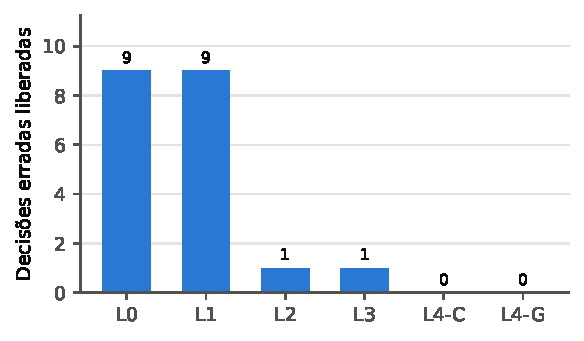
\includegraphics[width=0.6\linewidth]{fig_api_impacto.pdf}
\caption{Decisões erradas que chegariam à produção, somadas sobre os mutantes, por nível (L4-C: Claude; L4-G: GPT).}
\label{fig:impacto}
\end{figure}

%%%%%%%%%%%%%%%%%%%%%%%%%%%%%%%%%%%%%%
%%%%%%%%%%%% Seção 7  %%%%%%%%%%%%%%%%
%%%%%%%%%%%%%%%%%%%%%%%%%%%%%%%%%%%%%%
\section{Lacunas e Plano de Pesquisa}
\label{sec6:plano}

\textbf{Lacunas do estudo exploratório.} O protótipo mostra o mecanismo, mas deixa lacunas que o plano de pesquisa precisa fechar: (i) a escala é de brinquedo, com um serviço, cinco regras e mutantes escritos pelo autor; (ii) a anotação \code{@RegraPolitica} foi criada para o estudo e não existe em projetos reais, onde o vínculo entre contrato e código terá de vir do que já existe, como o \code{operationId}, as anotações do springdoc e o mapeamento das rotas nos \textit{controllers}; (iii) em APIs reais, boa parte da deriva é de esquema e de comportamento (códigos de \textit{status}, campos obrigatórios, restrições de validação e respostas de erro), e não apenas de texto de regra; (iv) falta comparar a abordagem com as ferramentas que as equipes já usam, como geração do contrato a partir do código, comparação de versões do contrato, teste baseado em esquema \cite{hatfield2022schemathesis} e contratos dirigidos pelo consumidor \cite{robinson2006cdc}; (v) o verificador lê Java com expressões regulares, o que não escala e explica o alarme falso de N07; e (vi) cada modelo foi executado uma vez, sem medir variação, custo ou latência, e sem um modelo aberto executado localmente, que seria necessário quando o código não pode sair da empresa; e (vii) a IA generativa só aponta e explica a divergência, sem ainda propor a correção.

\textbf{Questões de pesquisa.} A questão principal é: \textit{em que medida a IA generativa, combinada à rastreabilidade orientada por especificações, detecta a deriva entre contratos OpenAPI e o código de serviços Spring que as práticas usuais não detectam, e a que custo?} Ela se desdobra em quatro questões:
\begin{itemize}[noitemsep, topsep=3pt, leftmargin=1.5em]
  \item \textbf{QP1:} quais tipos de deriva entre contrato e código ocorrem na evolução de projetos Spring reais, e com que frequência?
  \item \textbf{QP2:} a verificação estrutural e a verificação semântica com LLM detectam mais derivas do que as práticas usuais (testes, checagem de esquema e comparação de contratos)?
  \item \textbf{QP3:} qual é o custo da verificação como portão de integração contínua (alarmes falsos, latência, \textit{tokens} e revisão humana)?
  \item \textbf{QP4:} como os resultados variam entre modelos, incluindo modelos abertos executados localmente, e entre execuções repetidas?
\end{itemize}

As hipóteses são direcionais: \textbf{H1}, a rastreabilidade SDD tem maior sensibilidade do que as práticas usuais; \textbf{H2}, a verificação semântica detecta derivas ressincronizadas que nenhuma verificação estrutural detecta; e \textbf{H3}, ela impõe custos mensuráveis, que dependem do modelo.

\textbf{Etapas.} O estudo segue as diretrizes de experimentação em Engenharia de Software de \cite{wohlin2012experimentation} e está organizado em cinco etapas, cada uma ligada às lacunas acima:
\begin{enumerate}[noitemsep, topsep=3pt, leftmargin=1.5em]
  \item \textit{Revisão sistemática} \cite{kitchenham2007slr} sobre evolução e documentação de APIs, teste de APIs REST, inconsistência entre código e documentação e uso de LLMs nessas tarefas.
  \item \textit{Corpus real} (lacunas i e iii): mineração de repositórios Spring Boot de código aberto que publicam contratos OpenAPI, identificando \textit{commits} em que contrato e código mudaram separadamente; as derivas encontradas serão rotuladas por dois avaliadores independentes, com medida de concordância, e servirão de base para operadores de mutação gerados sistematicamente.
  \item \textit{Ferramenta para projetos reais} (lacunas ii, iii, v e vii): reimplementação do verificador em Java, com JavaParser, como \textit{plugin} Maven e \textit{GitHub Action}; vínculo entre contrato e código por \code{operationId} e rotas, sem anotações próprias; \textit{fingerprint} sobre a árvore sintática, imune a renomeações; checagem de esquema, \textit{status} e validação (\textit{Bean Validation}); e geração, pelo LLM, de uma proposta de correção do contrato ou do código, anexada ao \textit{pull request} para aprovação humana (lacuna vii).
  \item \textit{Experimentos} (lacunas iv e vi): comparação com as ferramentas usuais sobre o mesmo corpus; vários LLMs, incluindo ao menos um modelo aberto local; execuções repetidas para medir variação; e medição de custo (latência p50/p95, \textit{tokens}, taxa de revisão humana).
  \item \textit{Análise}, com sensibilidade e precisão dos alertas por nível e por tipo de deriva. Intervalos de confiança serão estimados por \textit{bootstrap} agrupado por projeto \cite{efron1993bootstrap}, e comparações pareadas de detecção usarão o teste de McNemar \cite{mcnemar1947}, com correção para comparações múltiplas. Um estudo de caso com uma equipe de desenvolvimento \cite{runeson2009casestudy} poderá avaliar o portão em uso real.
\end{enumerate}

\textbf{Cronograma.} A Figura~\ref{fig:cronograma} apresenta o cronograma previsto para 24 meses.

\begin{figure}[!ht]
\centering
\resizebox{0.9\linewidth}{!}{
\begin{ganttchart}[
  hgrid, vgrid={*2{draw=none}, dotted},
  x unit=0.32cm, y unit chart=0.55cm,
  bar/.append style={fill=blue!25, draw=blue!60, line width=0.7pt, rounded corners=1pt},
  milestone/.append style={fill=red!50, draw=red!60},
  bar label font=\small, title label font=\small,
  bar height=0.55
]{1}{24}
  \gantttitle{Trimestres (24 meses)}{24}\\
  \gantttitlelist{1,...,8}{3}\\
  \ganttbar{Disciplinas obrigatórias}{1}{12}\\
  \ganttbar{Revisão sistemática}{1}{6}\\
  \ganttbar{Mineração do corpus e rotulagem}{5}{11}\\
  \ganttbar{Ferramenta em Java (Maven, CI)}{7}{14}\\
  \ganttmilestone{Qualificação}{12}\\
  \ganttbar{Experimentos com ferramentas e LLMs}{13}{18}\\
  \ganttbar{Análise e artigo}{17}{21}\\
  \ganttbar{Redação da dissertação}{18}{24}\\
  \ganttmilestone{Defesa}{24}
\end{ganttchart}}
\caption{Cronograma previsto.}
\label{fig:cronograma}
\end{figure}

%%%%%%%%%%%%%%%%%%%%%%%%%%%%%%%%%%%%%%
%%%%%%%%%%%% Seção 8  %%%%%%%%%%%%%%%%
%%%%%%%%%%%%%%%%%%%%%%%%%%%%%%%%%%%%%%
\section{Ameaças à Validade}
\label{sec7:ameacas}

Em relação à \textit{validade de construto}, \textit{fingerprints} e \textit{digests} verificam integridade, não significado, e o oráculo de cada deriva exige revisão independente. Quanto à \textit{validade interna}, mutantes escritos pelo autor do verificador introduzem viés de construção, e a instrução do verificador semântico foi escrita conhecendo os operadores, o que pode favorecer a detecção; o estudo confirmatório usará derivas reais e rótulos de terceiros, e as ferramentas de comparação serão configuradas segundo suas próprias recomendações. Quanto à \textit{validade externa}, um único serviço sintético não representa APIs reais, que têm mais rotas, mais regras e documentação menos estruturada; por isso o corpus será minerado de projetos de código aberto. Quanto à \textit{validade de conclusão}, os resultados com LLM vêm de uma única execução de cada modelo; o \textit{cache} garante a reprodução dessas respostas, mas não a estabilidade do modelo em novas execuções. Por fim, a política \textit{fail-closed} aumenta bloqueios, cujo custo para a equipe será medido e reportado.

%%%%%%%%%%%%%%%%%%%%%%%%%%%%%%%%%%%%%%
%%%%%%%%%%%% Seção 9  %%%%%%%%%%%%%%%%
%%%%%%%%%%%%%%%%%%%%%%%%%%%%%%%%%%%%%%
\section{Considerações Finais}
\label{sec8:final}

Este projeto trata de um problema comum na engenharia de APIs e difícil de perceber: o contrato OpenAPI, que os consumidores leem, e o código do serviço, que executa, deixam de dizer a mesma coisa sem que nenhum teste falhe. O \proj\ propõe amarrar requisitos, contrato e código numa especificação versionada e verificar esse vínculo como portão de integração contínua, com IA generativa para a parte que exige entender o texto. O protótipo mostra, em pequena escala, que as práticas usuais detectam metade das derivas injetadas, que a rastreabilidade estrutural chega a 10 de 12 ao custo de alarmes falsos em mudanças benignas, e que as derivas ressincronizadas, em que testes ou marcas são ajustados junto com a mudança, só são detectadas pela verificação semântica com LLM.

Do ponto de vista científico, o trabalho pretende contribuir na interseção entre engenharia de APIs, rastreabilidade e uso de LLMs em Engenharia de Software, com um estudo sobre ganhos, custos e limites da verificação de coevolução em projetos reais. Do ponto de vista prático, pretende oferecer às equipes que mantêm serviços Spring uma ferramenta que roda no \textit{pipeline} que elas já usam, sem substituir a revisão humana.

%%%%%%%%%%%%%%%%%%%%%%%%%%%%%%%%%%%%%%
%%%%%%%% Disponibilidade  %%%%%%%%%%%%
%%%%%%%%%%%%%%%%%%%%%%%%%%%%%%%%%%%%%%
\section*{Disponibilidade dos Artefatos}
{
\small
O protótipo está disponível em repositório público (\repourl). Esse material inclui: (i) o serviço Spring Boot de exemplo, com seus testes JUnit; (ii) as especificações e os contratos OpenAPI das versões 1 e 2; (iii) o verificador (pacote \code{apidrift}), com 30 testes automatizados que simulam o LLM e rodam sem rede, e a \textit{GitHub Action} do portão; (iv) os resultados brutos do estudo de mutações (\code{results/}) e os \textit{caches} com as respostas dos LLMs (\code{llm\_cache/}), que permitem refazer a Seção~\ref{sec5:preliminares} sem chave de API; e (v) o \textit{script} que gera as figuras deste texto.
}

%%%%%%%%%%%%%%%%%%%%%%%%%%%%
%%%%%%%%% Uso de IA %%%%%%%%
%%%%%%%%%%%%%%%%%%%%%%%%%%%%
\section*{Uso de Inteligência Artificial}
\label{Sec:IA}
{
\small
Em conformidade com o Código de Conduta para Autores da SBC, declara-se que ferramentas de IA foram utilizadas como apoio. O \textit{Claude} (Anthropic) foi utilizado como apoio à implementação do protótipo, à geração das figuras a partir dos resultados e à redação e organização deste texto. Separadamente, o Claude Opus 5.5 e o GPT-5.5 (OpenAI) são objetos do estudo, como os modelos avaliados no verificador semântico. O conteúdo científico, a verificação das referências e as conclusões apresentadas são de responsabilidade exclusiva do autor.
}

\bibliographystyle{sbc}
\bibliography{references}

\end{document}
